\section{Описание практической части}
\label{sec:Chapter4}

В рамках работы разработан и собран лабораторный прототип системы. Ниже описаны
передающий узел БПЛА, тракт обработки сигнала якоря, двухимпульсный метод
самокалибровки времени прихода, система питания и защиты от наводок, протокол
UWB-синхронизации узлов и результаты экспериментальной проверки приёмного тракта.

\subsection{Узел БПЛА (передающая часть)}
\label{sec:uav-node}

Узел БПЛА выполняет две задачи: излучение ультразвукового сигнала на частоте 25~кГц
и радиочастотную синхронизацию момента излучения с центральным узлом на платформе.
За каждый рабочий цикл узел излучает \textbf{пару идентичных импульсов} (пачек несущей)
с фиксированным разносом~--- этого требует двухимпульсный метод самокалибровки времени
прихода (раздел~\ref{sec:two-pulse}). Первый импульс является измерительным, и его старт
жёстко синхронизируется с радиосигналом; второму достаточно лишь стабильного разноса
относительно первого. Жёсткое совмещение моментов начала ультразвукового и радиоимпульса
является принципиальным требованием: при заданном уровне точности ToF на уровне миллиметра
случайное рассогласование между фактическим стартом акустического сигнала и
зафиксированным радиосинхросигналом не должно превышать нескольких микросекунд.

\subsubsection{Структурная схема}

В состав узла входят микроконтроллер ESP32-S3, сверхширокополосный (UWB) радиомодуль
DWM1000 (Decawave/Qorvo), счетверённый аналоговый ключ SN74HC4066N, мостовой драйвер
TC4427A и пьезоизлучатель Murata MA40S4S (рис.~\ref{fig:uav-block}).
ESP32-S3 средствами модуля MCPWM формирует непрерывную несущую 25~кГц в виде двух
строго противофазных меандров на выводах GPIO4 и GPIO5 и одновременно конфигурирует
DWM1000 по интерфейсу SPI. Открытие тракта несущей на драйвер выполняется аппаратно
сигналом EXTTXE радиомодуля.

\begin{figure}[h!]
\centering
\begin{tikzpicture}[
  blk/.style={draw, thick, rectangle, minimum width=2.6cm, minimum height=1.1cm,
              align=center, font=\small, inner sep=3pt},
  arr/.style={thick, ->}
]
\node[blk] (mcu)  at (0,    1.4) {ESP32-S3\\[-2pt]{\scriptsize $A$, $B$: 25\,кГц (противофаза)}};
\node[blk] (rf)   at (0,   -1.4) {DWM1000\\[-2pt]{\scriptsize 2 кадра/цикл}};
\node[blk] (sw)   at (4.8,  0)   {SN74HC4066\\[-2pt]{\scriptsize 2 ключа: $A$, $B$}};
\node[blk] (drv)  at (8.8,  0)   {TC4427A\\[-2pt]{\scriptsize драйвер (мост)}};
\node[blk] (pz)   at (12.4, 0)   {MA40S4S};
\draw[arr] (mcu.east) -| (sw.north);
\draw[arr] (rf.east)  -| (sw.south);
\draw[arr] (sw) -- (drv);
\draw[arr] (drv) -- (pz);
\draw[<->, thick] (mcu.south) -- (rf.north) node[midway, right, font=\scriptsize] {SPI};
\node[font=\scriptsize] at (2.6,  1.0) {2 канала};
\node[font=\scriptsize] at (2.6, -1.0) {EXTTXE};
\end{tikzpicture}
\caption{Структурная схема узла БПЛА: ESP32-S3 формирует два противофазных канала
несущей 25~кГц ($A$ и~$B$) для дифференциального возбуждения моста и управляет
радиомодулем DWM1000 по SPI; в момент старта UWB-пакета модуль аппаратно открывает
оба аналоговых ключа SN74HC4066 общим сигналом EXTTXE.}
\label{fig:uav-block}
\end{figure}

\subsubsection{Аппаратная синхронизация через EXTTXE}

Центральный узел вычисляет дальность по интервалу между приёмом UWB-кадра (общая метка
времени) и моментом детектирования ультразвукового импульса якорем. В идеале этот интервал
равен времени распространения звука; реально к нему добавляются задержки тракта, которые
по влиянию на точность ToF удобно разделить на три типа.

\textbf{Постоянные систематические задержки (безопасны).}
Это, прежде всего, задержка радиочастотной цепи DWM1000 от момента записи команды по SPI
до фактического подъёма сигнала EXTTXE~\cite{dw1000} (${\sim}150$~мкс на инициализацию синтезатора и
формирование RF-преамбулы), а также задержка распространения в антенне, задержка
переключения компаратора (${\sim}200$~нс) и обработки на приёмной стороне. Все они постоянны
от цикла к циклу и входят в одну аддитивную константу, определяемую при калибровке: при
вычитании она сокращается и на измеренную дальность не влияет. Поэтому важен не абсолютный
момент старта, а отсутствие в нём случайной составляющей.

\textbf{Случайные задержки (опасны).}
Программный запуск передачи в ESP32-S3 проходит через прерывания операционной системы
FreeRTOS. Время реакции на прерывание зависит от состояния планировщика, кэшей
инструкций и обработчиков более приоритетных прерываний; результирующий разброс
момента старта составляет 1--5~мкс. Он непредсказуем и не воспроизводится
от цикла к циклу, поэтому напрямую переходит в погрешность ToF: при $\Delta t = 1$~мкс
ошибка дальности $\Delta d = c\,\Delta t \approx 0{,}34$~мм. При требуемой точности
на уровне миллиметра такой джиттер недопустим и должен быть устранён.

\textbf{Зависящая от дальности систематика.}
Задержка срабатывания компаратора между истинным приходом и пересечением порога зависит от
амплитуды сигнала, а та убывает с расстоянием. Эта задержка постоянна для данной дистанции,
но меняется с дальностью, поэтому не сводится к калибровочной константе и не усредняется.
Она компенсируется отдельно~--- двухимпульсной самокалибровкой времени прихода
(раздел~\ref{sec:two-pulse}).

\textbf{Устранение случайного джиттера.}
Применяется аппаратный механизм отложенной передачи DWM1000 (\textit{Delayed TX}).
ESP32-S3 заранее, за несколько сотен микросекунд до требуемого момента, программирует
по SPI время старта; далее весь процесс ведёт встроенный радиочастотный таймер модуля
с шагом 15~пс. В заранее запрограммированный момент DWM1000 поднимает в высокий уровень
сигнал EXTTXE (вывод GPIO5, выведенный на внешние контакты модуля). Поскольку SPI-команда
подаётся заблаговременно, программный джиттер ESP32-S3 укладывается в окно ожидания и
не переходит на момент EXTTXE; стартом командует только аппаратный таймер.

Сигнал EXTTXE подаётся на разрешающие входы аналоговых ключей SN74HC4066N.
Непрерывная несущая 25~кГц с выводов ESP32-S3 попадает на драйвер только в активном
состоянии EXTTXE; до этого момента и после завершения пачки путь сигнала разорван.
Моменты физического начала ультразвукового излучения и UWB-передачи жёстко связаны
общим логическим фронтом; взаимный джиттер между ними определяется задержками
логических вентилей и не превышает 10~нс, что соответствует ошибке ToF
$\Delta d \approx 3{,}4$~мкм~--- пренебрежимо мало. Оба импульса пары формируются
двумя UWB-передачами за цикл (немедленной и отложенной), поэтому их взаимный разнос
$\Delta T$ задаётся кварцевым таймером DWM1000 и стабилен с точностью ${\sim}8$~нс;
измерительным служит первый импульс, второму достаточно этого стабильного разноса.

В начале каждой пачки формируется преамбула из нескольких пустых периодов несущей:
она поглощает время инициализации RF-цепи DWM1000 и переходные процессы
пьезопреобразователя и приёмного тракта; полезная часть пачки идёт после преамбулы.

\subsubsection{Управление мостом и активное гашение пьезоизлучателя}

Драйвер TC4427A построен по схеме полного моста (H-мост) и питает пьезопреобразователь
дифференциально, то есть напряжением между двумя своими выходами. Чтобы получить
двуполярное возбуждение, на оба входа драйвера приходят два противофазных сигнала $A$ и $B$
с выводов ESP32-S3 через два ключа SN74HC4066N: один ключ коммутирует сигнал ($A$) ко входу
$\text{IN}_A$ драйвера, второй~--- сигнал ($B$) ко входу $\text{IN}_B$. Общим разрешающим
сигналом для обоих ключей служит EXTTXE, что обеспечивает строго одновременное открытие
путей и сохраняет наносекундную привязку к UWB-пакету.

Пока EXTTXE активен (на время пачки), на входах драйвера присутствует противофазная пара
$A$/$B$: выходы моста формируют дифференциальный размах ${\pm}V_\text{DD}$ на излучателе~---
идёт излучение несущей.

После окончания пачки EXTTXE снимается, ключи SN74HC4066N размыкаются и отсоединяют несущую
от входов драйвера. Входы $\text{IN}_A$, $\text{IN}_B$ подтянуты к общему проводу резисторами
10~кОм, поэтому в паузе оба они оказываются в низком уровне, а оба выхода моста~--- на общем
проводе. Излучатель при этом замкнут через нижние ключи моста с малым сопротивлением
открытого канала ($R_{DS(\text{on})} \sim 0{,}5$~Ом).

Пьезоэлектрический преобразователь MA40S4S обладает высокой механической добротностью:
после прекращения возбуждения собственные колебания затухают за ${\sim}400$~мкс. Замыкание
излучателя в паузе диссипирует запасённую механическую энергию через сопротивление
$R_{DS(\text{on})}$~--- остаточные колебания гасятся активно за время порядка одного периода
несущей. Это устраняет «звон» между двумя импульсами пары и перед следующим циклом,
улучшая определение переднего фронта огибающей на приёме.

Управляющие входы двух неиспользуемых ключей микросхемы SN74HC4066N подтянуты к общему
проводу резисторами 10~кОм, гарантируя их закрытое состояние.

\FloatBarrier

\subsection{Узел якоря: обработка сигнала}

Цепь обработки сигнала каждого якоря включает четыре последовательных блока
(рис.~\ref{fig:anchor-block}): предусилитель~INA128P, усилитель~TL072CN
(два каскада: ФВЧ и ФНЧ) и демодулятор (детектор огибающей совместно с компаратором~LM311P).

Пьезоприёмник является механическим резонатором: любое акустическое воздействие~---
хлопок, удар, вибрация~--- преобразуется в затухающие колебания на той же частоте~25~кГц,
что и полезный сигнал. Поэтому полосовой фильтр не позволяет отличить полезный сигнал
от механического шума. Надёжное распознавание обеспечивается временным кодированием:
передатчик излучает пару пачек длительностью~${\sim}1$~мс каждая, а микроконтроллер
идентифицирует сигнал по характерному двухимпульсному шаблону во времени. Фильтр выполняет вспомогательную роль: подавляет
электрические помехи в схеме (наводки питания, ВЧ-мусор), что позволяет поднять
коэффициент усиления без перегрузки.

\begin{figure}[h!]
\centering
\resizebox{\textwidth}{!}{%
\begin{tikzpicture}[
  blk/.style={draw, thick, rectangle, minimum width=2.9cm, minimum height=1.4cm,
               align=center, font=\small, inner sep=4pt},
  arr/.style={thick, ->}
]
\node[blk] (pre) at (0,   0) {Предусилитель\\[-2pt]{\scriptsize INA128P,\;$G{\approx}25\text{--}100$}};
\node[blk] (amp) at (4.6, 0) {Усилитель\\[-2pt]{\scriptsize TL072CN,\;$K{\approx}64$}};
\node[blk] (dem) at (9.2, 0) {Демодулятор\\[-2pt]{\scriptsize огибающая + порог}};
\draw[arr] (-2.8,0) -- (pre) node[pos=0, left, font=\small, align=right] {УЗ\\приёмник};
\draw[arr] (pre) -- (amp);
\draw[arr] (amp) -- (dem);
\draw[arr] (dem) -- ++(2.4,0) node[right, font=\small] {МК};
\end{tikzpicture}%
}
\caption{Структурная схема цепи обработки сигнала якоря}
\label{fig:anchor-block}
\end{figure}

\subsubsection{Предусилитель --- INA128P}

На первом каскаде применяется инструментальный усилитель INA128P с дифференциальным входом (рис.~\ref{fig:ina128}).
Высокое выходное сопротивление пьезоприёмника обусловливает подключение резисторов
$1$~МОм от каждого входа на землю для задания тока смещения; конденсатор~100~пФ между
входами срезает высокочастотные наводки на входных проводах.
Коэффициент усиления задаётся резистором $R_g$ между выводами RG (выводы~1 и~8), который
образован последовательным соединением постоянного резистора $R_1 = 470$~Ом и подстроечного
$RP_1 = 1{,}5$~кОм ($R_g = R_1 + RP_1$):
\[
G = 1 + \frac{50\,\text{кОм}}{R_g}.
\]
Регулировка $RP_1$ изменяет $R_g$ в диапазоне 470--1970~Ом, что обеспечивает $G \approx 26\text{--}107$
и позволяет подстраивать усиление под конкретный экземпляр пьезоприёмника без изменения схемы.
Питание~--- $\pm12$~В, вывод REF подключён к аналоговой земле.

\begin{figure}[h!]
\centering
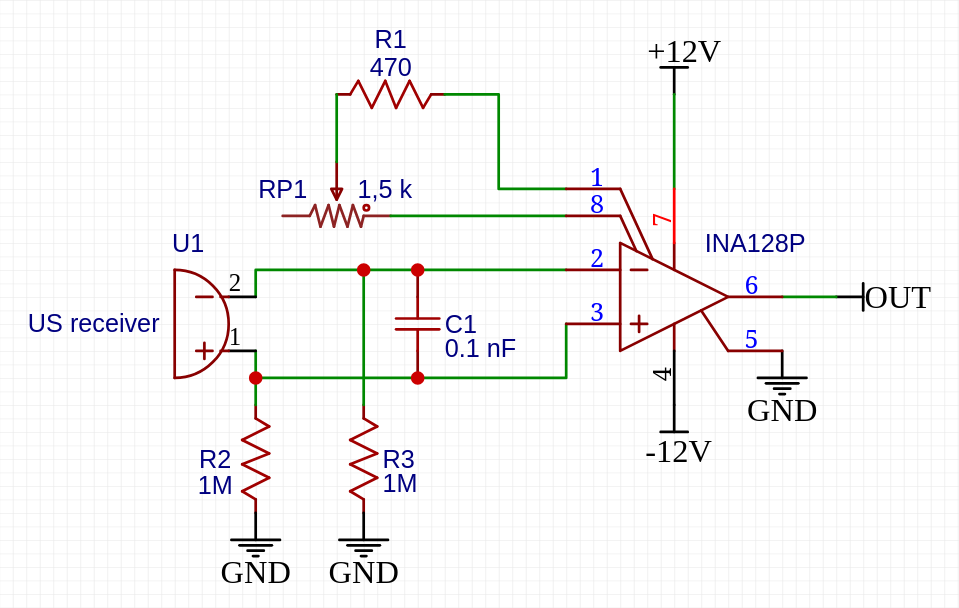
\includegraphics[width=0.75\textwidth]{images/ina_cascade.png}
\caption{Схема предусилителя INA128P}
\label{fig:ina128}
\end{figure}

\subsubsection{Усилитель --- TL072CN}

Оба операционных усилителя микросхемы TL072CN (U1.1 и U1.2) включены как неинвертирующие усилители (рис.~\ref{fig:tl072}).
Цепь обратной связи каждого каскада образована резисторами $R_f = 39$~кОм ($R_2$, $R_4$)
и $R_\text{вх} = 3{,}9$~кОм ($R_5$, $R_6$), что даёт одинаковый коэффициент усиления:
\[
K = 1 + \frac{R_f}{R_\text{вх}} = 1 + \frac{39}{3{,}9} = 11.
\]
Полосовая характеристика формируется входными RC-фильтрами обоих каскадов, частоты среза которых
расположены по краям рабочей полосы вокруг частоты 25~кГц.

\textbf{ОУ-A --- U1.1 (входной ФВЧ, $f_c \approx 22$~кГц).}
На неинвертирующий вход сигнал подаётся через фильтр верхних частот: конденсатор~$C_1 = 330$~пФ
последовательно с источником, резистор~$R_1 = 22$~кОм на землю:
\[
f_{c,A} = \frac{1}{2\pi R_1 C_1} \approx 22\text{ кГц.}
\]

\textbf{ОУ-B --- U1.2 (входной ФНЧ, $f_c \approx 27$~кГц).}
На неинвертирующий вход сигнал подаётся через фильтр нижних частот: резистор~$R_3 = 20$~кОм
последовательно с источником, конденсатор~$C_2 = 300$~пФ на землю:
\[
f_{c,B} = \frac{1}{2\pi R_3 C_2} \approx 27\text{ кГц.}
\]

На частоте 25~кГц оба фильтра работают в переходной зоне: ОУ-A --- незначительно выше своей частоты среза,
ОУ-B --- незначительно ниже.
Амплитудное ослабление на 25~кГц составляет ${\approx}0{,}75$ для входного ФВЧ (ОУ-A) и
${\approx}0{,}73$ для входного ФНЧ (ОУ-B), так что эффективный коэффициент каждого каскада
$K_\text{эфф} \approx 11 \cdot 0{,}74 \approx 8$, а суммарный коэффициент двух каскадов~$\approx 64$.
При частотах существенно ниже~22~кГц или выше~27~кГц один из каскадов вносит значительно большее
ослабление, поэтому суммарный коэффициент резко убывает~---
каскады совместно действуют как полосовой усилитель с центральной частотой 25~кГц.

\begin{figure}[h!]
\centering
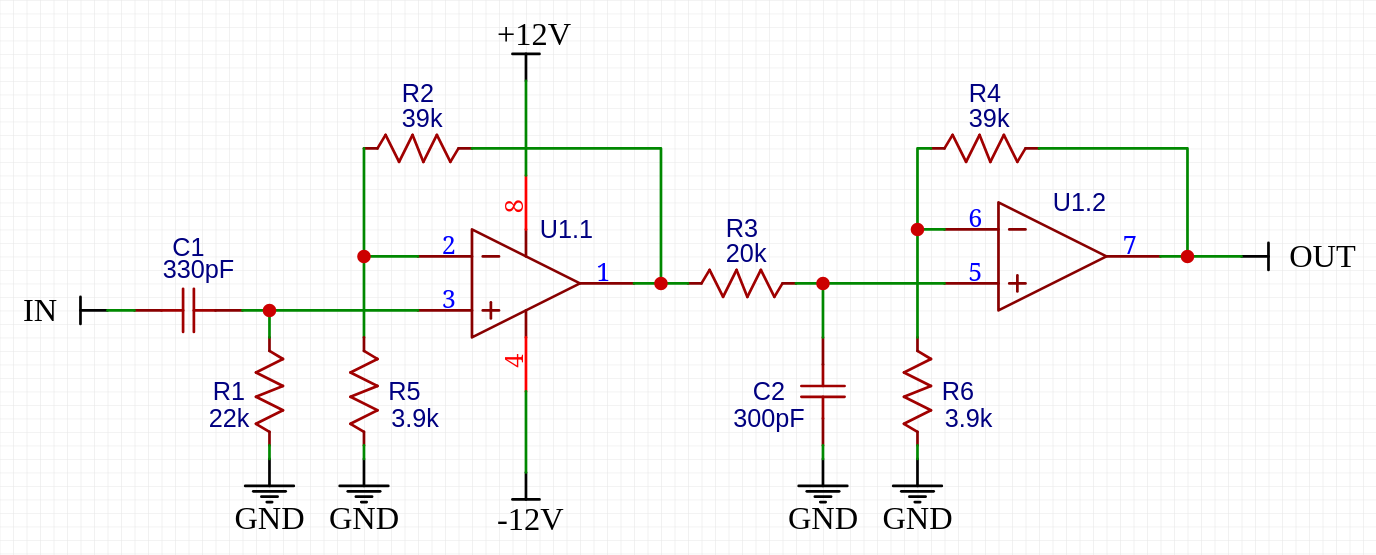
\includegraphics[width=\textwidth]{images/tl_cascade.png}
\caption{Каскады усилителя TL072CN: ОУ-A (U1.1)~--- неинвертирующий усилитель с входным ФВЧ
($f_c{\approx}22$\,кГц, $K_A{=}11$), ОУ-B (U1.2)~--- с входным ФНЧ ($f_c{\approx}27$\,кГц, $K_B{=}11$).
Питание $\pm12$\,В.}
\label{fig:tl072}
\end{figure}

\subsubsection{Демодулятор}

Демодулятор преобразует переменный сигнал 25~кГц в логический уровень для микроконтроллера
и состоит из детектора огибающей и быстрого компаратора с гистерезисом (рис.~\ref{fig:det-cmp}).

Детектор огибающей построен на германиевом диоде Д9, накопительном конденсаторе
$C_3 = 22$~нФ и разрядном резисторе $R_3 = 20$~кОм на землю; постоянная времени разряда:
\[
\tau = R_3 C_3 = 20\cdot10^{3} \cdot 22\cdot10^{-9} \approx 0{,}44\text{ мс.}
\]
Заряд конденсатора идёт через открытый диод с малым сопротивлением, поэтому передний фронт
огибающей повторяет начало пакета без задержки. Постоянная разряда выбрана из двух условий.
С одной стороны, она должна быть много больше периода несущей
($\tau \gg 1/(2\pi f_{\text{нес}}) \approx 6$~мкс), чтобы полностью сгладить заполнение и
получить гладкую огибающую. С другой~--- много меньше межимпульсного зазора
($\tau \ll 2$~мс), чтобы огибающая успевала вернуться к базовой линии между двумя импульсами
пары: при $\tau \approx 0{,}44$~мс за время зазора огибающая спадает в $e^{-2/0{,}44}\approx 1\%$,
так что второй импульс детектируется с чистого фронта~--- это необходимо для двухимпульсной
самокалибровки (раздел~\ref{sec:two-pulse}). Подавление более поздних эхо-сигналов
обеспечивается не постоянной времени детектора, а программным гейтом: микроконтроллер
принимает только первый приход в каждом цикле, а позднейшие отражения отбрасывает по времени.
Германиевый диод Д9 предпочтительнее кремниевого: его падение в открытом состоянии
${\sim}0{,}2$~В против ${\sim}0{,}6$~В у 1N4148 даёт выигрыш чувствительности
${\sim}0{,}4$~В, что существенно для слабых сигналов на максимальной дальности.

Компаратор LM311P выбран взамен медленных операционных усилителей общего назначения
(LM358) и компараторов LM393: его задержка переключения составляет ${\sim}200$~нс
против ${\sim}1{,}3$~мкс у LM393, что вносит соответствующую погрешность ToF
$\Delta d = c\,\Delta t \approx 70$~мкм~--- существенно ниже погрешности детектирования
переднего фронта. LM311P имеет выход с открытым коллектором (вывод~7), сигнал с которого
подаётся на вход микроконтроллера; высокий логический уровень формируется подтягивающим
резистором на стороне микроконтроллера. Питание $+5$~В подаётся на вывод~8, вывод~4 соединён
с общей логической землёй.

Порог срабатывания задаётся делителем напряжения $R_2 = 100$~кОм (на $+5$~В) и
$R_1 = 5$~кОм (на землю), подключённым к инвертирующему входу:
\[
V_{\text{ref}} = 5\,\text{В} \cdot \frac{R_1}{R_1 + R_2}
= 5 \cdot \frac{5}{105} \approx 0{,}24\text{ В,}
\]
что соответствует уровню ${\sim}10\%$ от пиковой амплитуды огибающей при максимальной
дальности.
Положительная обратная связь резистором $R_4 = 1$~МОм с выхода на неинвертирующий
вход создаёт небольшой гистерезис и исключает дребезг при переходе огибающей через порог.

\begin{figure}[h!]
\centering
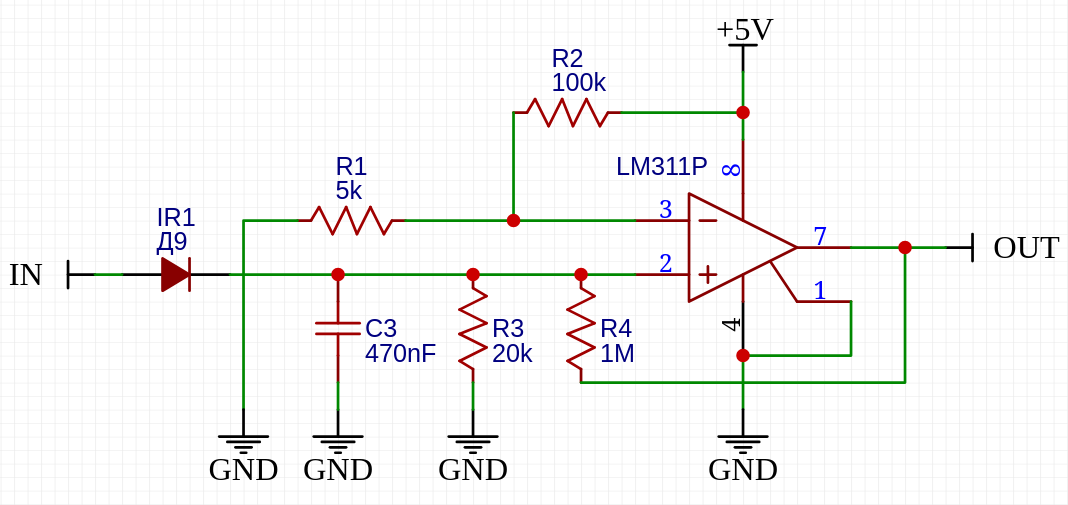
\includegraphics[width=0.95\textwidth]{images/detector_comporator.png}
\caption{Демодулятор: детектор огибающей на германиевом диоде Д9 и компаратор LM311P
с открытым коллектором; порог задаётся делителем $R_1$, $R_2$, гистерезис~--- резистором $R_4$}
\label{fig:det-cmp}
\end{figure}
\FloatBarrier

\subsubsection{Самокалибровка времени прихода: двухимпульсный метод}
\label{sec:two-pulse}

Компаратор фиксирует момент $t_c$ пересечения огибающей фиксированного порога $V_{th}$,
тогда как физическим моментом прихода прямой волны служит \emph{начало роста амплитуды}~$t_0$.
Огибающая нарастает за конечное время (измеренное время фронта ${\approx}0{,}2$~мс,
см.\ раздел~\ref{sec:exp}), поэтому компаратор срабатывает позже истинного прихода
на величину
\[
\delta = t_c - t_0 \approx \tau\,\frac{V_{th}}{V_{\max}},
\]
где $\tau$~--- характерное время нарастания, $V_{\max}$~--- амплитуда огибающей.
Поскольку амплитуда сигнала убывает с расстоянием, задержка $\delta$ у дальних якорей
больше, чем у ближних: для слабого сигнала на пределе дальности порог достигается почти
у вершины огибающей и $\delta$ приближается к полному времени фронта (${\sim}0{,}2$~мс,
что эквивалентно ${\sim}70$~мм по дальности), тогда как для сильного сигнала $\delta$
составляет единицы миллиметров. Это не случайный шум, а \textbf{систематическое смещение},
зависящее от дальности: оно не усредняется и искажает геометрию трилатерации, поэтому
требует не фильтрации, а компенсации в каждом измерении.

Для этого передатчик излучает \textbf{пару идентичных импульсов} с известным разносом
$\Delta T_{tx}=3$~мс (импульс ${\sim}1$~мс и зазор ${\sim}2$~мс, рис.~\ref{fig:two-pulse}). Компаратор срабатывает
на оба импульса, давая метки $t_{c1}$ и $t_{c2}$ (аппаратный захват таймером с разрешением
12,5~нс). Вокруг ожидаемого прихода второго импульса ($t_{c1}+\Delta T_{tx}$) микроконтроллер
открывает короткое окно АЦП (${\approx}500$~мкс, однократный запуск), оцифровывает нарастающий
фронт его огибающей и восстанавливает по нему старт роста $t_{0,2}$ (экстраполяцией фронта
к базовой линии). Измеренная разность
\[
\delta = t_{c2} - t_{0,2}
\]
и есть смещение компаратора. Так как оба импульса проходят один и тот же путь и разнесены
на интервал, много меньший времени изменения геометрии, их амплитуды, а значит и $\delta$,
совпадают. Несмещённую оценку времени прихода \emph{первого} импульса тогда даёт
\[
t_{\text{ToA}} = t_{c1} - \delta = t_{0,1}.
\]

Подход выбран ради простоты и устойчивости. Окно АЦП работает в однократном режиме, без
непрерывной потоковой оцифровки и DMA, что заметно упрощает прошивку по сравнению с
согласованной фильтрацией непрерывного потока. Переотражения подавляются автоматически:
эхо одинаково на обоих импульсах и потому не искажает разность $\delta$. Разность
$t_{c2}-t_{c1}$ служит дополнительной проверкой качества: её отклонение от $\Delta T_{tx}$
сигнализирует о сбое (помеха, пропуск импульса) и позволяет забраковать отсчёт. Наконец,
температурный дрейф добротности пьезопреобразователя (а с ней и времени фронта~$\tau$)
не требует калибровки~--- $\delta$ измеряется заново в каждом цикле.

\begin{figure}[h!]
\centering
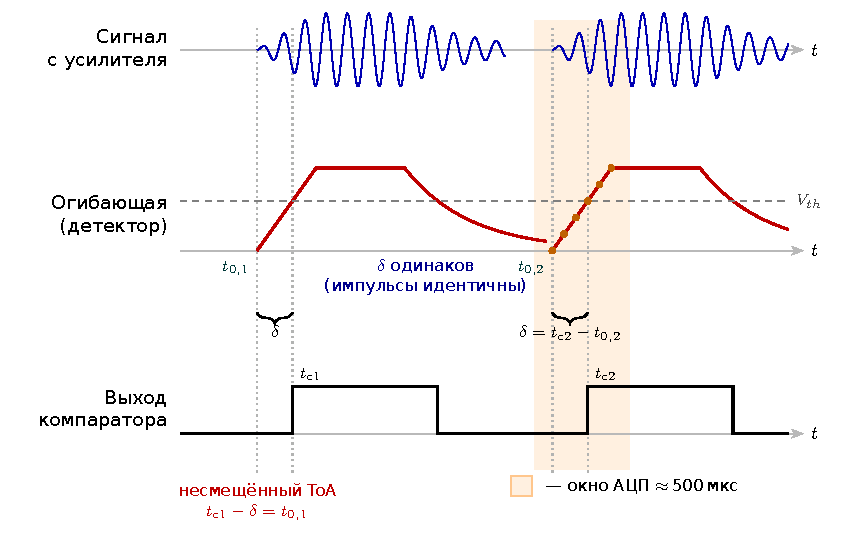
\includegraphics[width=\textwidth]{images/two_pulse_toa.pdf}
\caption{Двухимпульсная самокалибровка времени прихода: сигнал с усилителя (две идентичные
пачки 25~кГц), огибающая с порогом $V_{th}$ и выход компаратора. Реальный приход~$t_0$~---
начало роста амплитуды; компаратор срабатывает позже на~$\delta$. По окну АЦП на втором
импульсе измеряется $\delta=t_{c2}-t_{0,2}$ и переносится на первый: $t_{\text{ToA}}=t_{c1}-\delta$.
Порог $V_{th}$ показан завышенным относительно реального (${\sim}10\%$ от пика)
для наглядности зазора~$\delta$.}
\label{fig:two-pulse}
\end{figure}
\FloatBarrier

\subsubsection{Бюджет случайной ошибки измерения дальности}
\label{sec:error-budget}

Двухимпульсная калибровка устраняет систематическое смещение $\delta$ (до ${\sim}70$~мм
у дальних якорей), поэтому остаточная погрешность времени прихода~--- \emph{случайная}.
Оценим её бюджет и получим СКО измерения дальности $\sigma_d$, входящее в расчёт точности
позиционирования.

\textbf{Джиттер порога (доминирующий вклад).} Компаратор фиксирует момент $t_c$ пересечения
огибающей $V(t)$ с порогом $V_{th}$. Аддитивный шум с СКО $\sigma_n$ смещает этот момент;
линеаризуя условие $V(t_c)=V_{th}$ в окрестности срабатывания, получаем
$$
\sigma_t = \frac{\sigma_n}{\left|\,\mathrm{d}V/\mathrm{d}t\,\right|_{t_c}}.
$$
Огибающая нарастает от нуля до амплитуды $V_{\max}$ за время фронта $\tau$, поэтому вблизи
низкого порога (${\sim}10\%$ от пика) крутизна близка к максимальной,
$\mathrm{d}V/\mathrm{d}t \approx V_{\max}/\tau$. Отсюда
$$
\sigma_t \approx \tau\,\frac{\sigma_n}{V_{\max}} = \frac{\tau}{\mathrm{SNR}},
\qquad
\sigma_{d,\mathrm{th}} = c\,\sigma_t \approx \frac{c\,\tau}{\mathrm{SNR}},
$$
где $\mathrm{SNR}=V_{\max}/\sigma_n$~--- амплитудное отношение сигнал/шум. При измеренном
фронте $\tau\approx0{,}2$~мс (откуда $c\tau\approx69$~мм), наблюдаемой амплитуде
$V_{\max}\approx1{,}5$~В и остаточном фоне $\sigma_n\lesssim50$~мВ в отсутствие излучателя
($\mathrm{SNR}\approx30$) получаем $\sigma_{d,\mathrm{th}}\approx2{,}3$~мм.

\textbf{Прочие независимые вклады.} Складываются с доминирующим в квадратуре:
\begin{itemize}
  \item квантование захвата таймера у каждого якоря: шаг $\Delta t=12{,}5$~нс даёт
        $c\,\Delta t/\sqrt{12}\approx1$~мкм;
  \item атмосферная турбулентность: трассы к якорям почти совпадают и расходятся лишь
        у платформы, поэтому их общая часть систематична, а случайна лишь дифференциальная
        составляющая~--- на ${\sim}25$~м в спокойном воздухе $\lesssim1$~мм.
\end{itemize}

\textbf{Что не входит.} Погрешности, \emph{общие} для всех якорей в пределах одного цикла
измерений~--- прежде всего оценка скорости звука по датчику BME280 и общий момент старта
пачки (UWB-синхронизация),~--- являются \emph{систематическими}: они синхронно масштабируют
или сдвигают все измеренные дальности и потому не размножаются коэффициентом GDOP как
независимые ошибки. Их вклад учитывается отдельно, при оценке систематического смещения
(${\sim}3$~см от остаточной погрешности скорости звука), и в случайный бюджет $\sigma_d$
не включается. В $\sigma_d$ входят только независимые по якорям источники.

\textbf{Итог.} Складывая независимые вклады в квадратуре,
$$
\sigma_d=\sqrt{\sigma_{d,\mathrm{th}}^2+\sigma_{\mathrm{turb}}^2}
\approx\sqrt{2{,}3^2+1^2}~\text{мм}\approx2{,}5~\text{мм}.
$$
Бюджет полностью определяется акустическим джиттером порога. В дальнейших оценках
принимается округлённое с запасом значение $\sigma_d=3$~мм. На пределе дальности, где
амплитуда падает до $V_{\max}\approx1$~В ($\mathrm{SNR}\approx20$), $\sigma_{d,\mathrm{th}}$
возрастает до ${\sim}4$~мм, что соответствует ошибке положения ${\sim}7$~см.

\FloatBarrier

\subsection{Узел якоря: питание и защита от наводок}
\label{sec:anchor-power}

Описанный выше тракт обработки сигнала с полным усилением ${\sim}64\text{--}77$~дБ
особо чувствителен к наводкам по цепям питания: ничтожный уровень помехи на входной
шине $\pm 12$~В усиливается операционными усилителями наравне с полезным сигналом
и при недостаточной фильтрации способен полностью замаскировать сигнал
полезной частоты 25~кГц.

Эта чувствительность приобретает особое значение в полевой эксплуатации.
Приёмная подсистема состоит из четырёх якорей, разнесённых по периметру платформы
в выбранной по условиям GDOP геометрии. Каждый якорь получает $+24$~В от центрального
узла отдельным проводом; вместе с обратными сигнальными линиями от компараторов
это образует пучок из нескольких протяжённых (несколько метров) проводных трасс,
проходящих по корпусу платформы.
Эти линии работают как антенны для широкополосных электромагнитных помех
от штатного оборудования платформы~--- дизельного электрогенератора и силовых
инверторов 400~В,~--- и являются основным каналом проникновения наводок к якорям.

Применяется трёхуровневая стратегия защиты: гальваническая развязка изолированным
DC/DC-преобразователем, входная и выходная LC-фильтрация шин питания, локальная развязка
по питанию каждой микросхемы.

\subsubsection{Изолированный преобразователь A2412S-2WR3}

Питание усилителя осуществляется от изолированного преобразователя Mornsun A2412S-2WR3
со следующими параметрами:
\begin{itemize}
    \item вход --- $21{,}6\text{--}26{,}4$~В постоянного тока (номинал 24~В);
    \item выход --- $\pm 12$~В постоянного тока, ток нагрузки до 83~мА на каждую шину
          при суммарной выходной мощности 2~Вт;
    \item напряжение изоляции вход/выход --- 1500~В постоянного тока.
\end{itemize}

Преобразователь полностью развязывает аналоговую землю усилителя (INA128P и оба ОУ
TL072CN) от шины питания платформы. Изоляция на уровне 1500~В исключает протекание
паразитных токов по контуру «платформа~--~длинный кабель~--~якорь» и качественно
надёжнее любого фильтрационного решения, поскольку отсекает помеху гальванически,
а не подавляет её на конкретных частотах.

\subsubsection{Входной фильтр шины 24\,В}

Питание подаётся от центрального узла платформы по экранированному кабелю; экран
заземляется только на стороне центра (одностороннее заземление --- исключает
образование земляных петель). На входе якоря установлен двухзвенный фильтр
(рис.~\ref{fig:anchor-power}): ферритовое кольцо ($2$--$3$ витка провода 24~В)
подавляет высокочастотные наводки синфазного типа; последующее $LC$-звено на дросселе
EC24-101K (100~мкГн), электролитическом конденсаторе 100~мкФ\,$\times$\,35~В и
керамическом конденсаторе 100~нФ выполняет дифференциальную фильтрацию коммутационных
импульсов и сглаживает просадку питания при пуске преобразователя.

\subsubsection{Выходные LC-фильтры шин $\pm 12$\,В}

Собственная частота коммутации преобразователя A2412S-2WR3 составляет ${\sim}100$~кГц,
что лежит выше рабочей полосы усилителя, но в пределах полосы пропускания операционных
усилителей INA128P и TL072CN и потому подавляется отдельно. Для подавления коммутационного
шума на каждой выходной шине установлен $LC$-фильтр на дросселе EC24-100K (10~мкГн)
и параллельной паре конденсаторов 10~мкФ\,$\times$\,35~В (электролит) и 100~нФ (керамика).
На шине $-12$~В электролитический конденсатор устанавливается в инвертированной полярности
(плюс к общему проводу).

\begin{figure}[h!]
\centering
\begin{tikzpicture}[
  blk/.style={draw, thick, rectangle, minimum width=2.4cm, minimum height=1.0cm,
              align=center, font=\small, inner sep=3pt},
  flt/.style={draw, thick, rectangle, minimum width=2.0cm, minimum height=1.0cm,
              align=center, font=\scriptsize, inner sep=3pt, fill=black!4},
  arr/.style={thick, ->}
]
\node[font=\small] (in)   at (-1.6, 0)   {$+24$\,В};
\node[flt]         (fer)  at (1.0,  0)   {Феррит\\(синф.)};
\node[flt]         (lc1)  at (3.8,  0)   {$L_1\,C_1$\\100\,мкГн / 100\,мкФ};
\node[blk]         (dcdc) at (7.2,  0)   {A2412S-2WR3\\[-2pt]{\scriptsize изол.\ DC/DC}};
\node[flt]         (lcp)  at (10.6,  1.1) {$L_2\,C_2$\\10\,мкГн / 10\,мкФ};
\node[flt]         (lcm)  at (10.6, -1.1) {$L_2\,C_2$\\10\,мкГн / 10\,мкФ};
\node[font=\small] (vp)   at (13.2,  1.1) {$+12$\,В};
\node[font=\small] (vm)   at (13.2, -1.1) {$-12$\,В};
\draw[arr] (in)   -- (fer);
\draw[arr] (fer)  -- (lc1);
\draw[arr] (lc1)  -- (dcdc);
\draw[arr] (dcdc.east) |- (lcp);
\draw[arr] (dcdc.east) |- (lcm);
\draw[arr] (lcp) -- (vp);
\draw[arr] (lcm) -- (vm);
\end{tikzpicture}
\caption{Схема питания узла якоря: входной фильтр (феррит\,+\,$LC$) перед изолированным
преобразователем A2412S-2WR3 и индивидуальные $LC$-фильтры на выходах $\pm 12$\,В}
\label{fig:anchor-power}
\end{figure}

\subsubsection{Топология земли}

Аналоговая земля усилителя GND$_{\text{из}}$ и логическая земля компаратора LM311P
и линии связи с центральным узлом GND$_{\text{л}}$ выполнены раздельно. Питание
логической части $+5$~В формируется отдельным линейным стабилизатором 7805 от шины
24~В, не проходя через изолированный преобразователь. Соединение GND$_{\text{из}}$ и
GND$_{\text{л}}$ выполнено в одной точке у компаратора (звёздная топология); эта точка
соединяется с землёй центрального узла одним проводом.

Звёздная топология исключает образование замкнутых контуров по земле, по которым
могли бы протекать паразитные токи от наводок и собственного коммутационного шума
DC/DC. Развязка по питанию каждой микросхемы (керамика 100~нФ возле каждого вывода
питания INA128P, TL072CN и LM311P) подавляет высокочастотные помехи на локальном уровне.

\FloatBarrier

\subsection{Протокол UWB-линка и синхронизация узлов}
\label{sec:protocol}

Узел БПЛА и центральный (наземный) узел связаны точка-точка по UWB-каналу
(DWM1000). Узел БПЛА выступает \emph{ведущим} (инициирует обмен и задаёт тайминг),
центральный~--- \emph{ведомым} (реактивно отвечает на принятый кадр). Канал
полудуплексный, поэтому ведущий шлёт запрос и слушает ответ, а ведомый отвечает.
Запуск построен по стадиям: ни один узел не переходит к работе вслепую, пока
предыдущая стадия явно не подтверждена.

\subsubsection{Стадии запуска}

\begin{enumerate}
\item \textbf{Самотест.} Каждый узел проверяет свой DWM1000 (чтение
  DEV\_ID $=$ \texttt{0xDECA0130} и инициализация). Провал~--- фатальное состояние
  с диагностикой.
\item \textbf{Рукопожатие.} БПЛА шлёт \texttt{PING}, центр отвечает \texttt{PONG}:
  подтверждается, что UWB-канал в принципе рабочий.
\item \textbf{Конфигурация.} БПЛА передаёт свой тайминг (частоты несущей и пакетов,
  длительности импульса и зазора, разнос стартов $\Delta T$); центр подстраивает
  окна детектирования \emph{с запасом} и отвечает \texttt{CONFIG\_ACK}. Это
  подтверждение служит точкой рандеву: центр переходит в режим ожидания первого
  рабочего пакета, а БПЛА получает разрешение начать рабочий цикл.
\item \textbf{Рабочий цикл.} БПЛА непрерывно шлёт пакеты \texttt{DATA} на $10$~Гц
  синхронно с ультразвуковыми парами; центр на каждый пакет отвечает квитанцией.
\end{enumerate}

Отдельная стадия проверки якорей не выделяется: исправность якоря наблюдаема прямо
в рабочем цикле (отсутствие отметки от якоря${=}$нет измерения), а её результат
центр сообщает в квитанции (маска живых якорей). Если живых якорей меньше минимума
для трилатерации ($3$ на плоскости, $4$ в пространстве), центр выдаёт признак
«нет решения» вместо заведомо неверной координаты.

\subsubsection{Установление первой позиции}

При частоте пакетов $f_\text{п}{=}10$~Гц однозначно (без целочисленной
неопределённости номера цикла) измеряется дальность лишь до
\[
R_\text{одн}=\frac{c}{f_\text{п}}=\frac{343}{10}\approx 34{,}3~\text{м},
\]
тогда как протокол проектируется с запасом на дистанции до $100$~м (целевые рабочие~---
$40$--$50$~м): на большей дальности время пролёта превышает период пакетов, и в воздухе
одновременно находится более одной ультразвуковой пары. Для однозначного старта применяется приём \emph{изоляции
первого пакета}. После \texttt{CONFIG\_ACK} БПЛА выдерживает паузу
\[
\tau \ge \frac{R_\text{макс}}{c}=\frac{100}{343}\approx 0{,}29~\text{с}\quad
(\text{принято }0{,}3~\text{с}),
\]
в течение которой несущая выключена и акустический эфир полностью очищается от
прежних сигналов. Затем БПЛА начинает штатную передачу $10$~Гц. Первый пакет
изолирован снизу тишиной длиной $\tau$, поэтому первое акустическое прибытие после
паузы для каждого якоря заведомо принадлежит именно ему (более поздние пакеты
приходят позже и не мешают), и его время пролёта измеряется однозначно на любой
дистанции до $100$~м. Далее номер цикла удерживается по непрерывности: за период
$0{,}1$~с БПЛА не смещается на десятки метров, поэтому соответствие
«пакет\,$\leftrightarrow$\,приём» отслеживается без потери. До установления первого
однозначного отсчёта центр помечает позицию как невалидную.

\subsubsection{Устойчивость к перезагрузке}

Стадия узла кодируется типом его ответного кадра (\texttt{PONG}~--- рукопожатие,
\texttt{CONFIG\_ACK}~--- конфигурация, квитанция~--- рабочий цикл), что позволяет
обнаружить рассогласование без отдельного поля. Если узел получает от партнёра
ответ, соответствующий \emph{более ранней} стадии (партнёр перезагрузился), либо
не получает ответа в течение $N$ пакетов подряд (канал потерян), он возвращается к
рукопожатию, после чего обе стороны заново проходят стадии. Инициатором подъёма
всегда выступает БПЛА, поэтому взаимная блокировка исключена: даже если БПЛА ещё
считает себя в рабочем цикле, перезагрузившийся центр ответит кадром стадии
рукопожатия, и БПЛА сам опустится. Одиночные потери пакетов на сброс не влияют~---
они компенсируются предсказанием фильтра, а сброс инициирует лишь устойчивая
регрессия стадии или продолжительная тишина. Перезагрузка БПЛА восстанавливается
бесшовно (центр продолжает счёт), перезагрузка центра требует повторного
установления первой позиции (${\sim}1$~с).

\subsubsection{Формат кадров}

Все кадры начинаются общей трёхбайтовой шапкой: признак системы
\texttt{magic}${=}$\texttt{0x55}, версия протокола \texttt{ver} и тип \texttt{type}.
Контрольную сумму (2~байта) добавляет аппаратно сам DWM1000, в полезную нагрузку
она не входит. Перечень сообщений приведён в таблице~\ref{tab:uwb-msgs}.

\begin{table}[h!]
\centering
\caption{Сообщения протокола UWB-линка}
\label{tab:uwb-msgs}
\small
\begin{tabular}{@{}llccp{5.9cm}@{}}
\toprule
Сообщение & Код & Направление & Стадия & Назначение \\ \midrule
\texttt{PING}        & \texttt{0x01} & БПЛА\,$\to$\,центр & рукопожатие  & проверка работоспособности UWB-канала \\
\texttt{PONG}        & \texttt{0x02} & центр\,$\to$\,БПЛА & рукопожатие  & ответ «канал жив» \\
\texttt{CONFIG}      & \texttt{0x03} & БПЛА\,$\to$\,центр & конфигурация & объявление тайминга передатчика \\
\texttt{CONFIG\_ACK} & \texttt{0x04} & центр\,$\to$\,БПЛА & конфигурация & «принято, ожидаю первый пакет» \\
\texttt{DATA}        & \texttt{0x06} & БПЛА\,$\to$\,центр & рабочий цикл & рабочий пакет, синхронный с УЗ-парой \\
\texttt{ACK}         & \texttt{0x05} & центр\,$\to$\,БПЛА & рабочий цикл & квитанция: стадия, маска якорей, валидность фикса \\
\bottomrule
\end{tabular}
\end{table}

\FloatBarrier

\subsection{Результаты экспериментальной проверки приёмного тракта}
\label{sec:exp}

\textbf{Дальность приёма.}
Уверенный приём сигнала достигнут на расстоянии~${\approx}40$~м при амплитуде на выходе
усилительного тракта~$1\text{--}2$~В, что обеспечивает надёжное срабатывание компаратора.
Эта дистанция ограничена размерами площадки испытаний, а не самой системой: сохраняющийся
запас по амплитуде и согласие с теоретической оценкой (раздел~\ref{sec:max-range})
показывают, что рабочая дальность выше и достигает целевых $40$--$50$~м.

\textbf{Разрешение пары импульсов.}
Передний фронт огибающей нарастает за~${\approx}0{,}2$~мс~--- достаточно круто для точного
определения времени прихода. Между двумя импульсами пары огибающая успевает вернуться к
базовой линии, поэтому оба импульса детектируются раздельно~--- необходимое условие
двухимпульсной самокалибровки (раздел~\ref{sec:two-pulse}).

Полученные результаты подтверждают работоспособность приёмного тракта: сигнал уверенно
принимается на рабочих дистанциях и разрешается в пару импульсов, на которой строится
измерение времени прихода. Тем самым предложенная схема применима для определения координат.

\FloatBarrier
